\documentclass[mathserif,serif]{beamer}
\usepackage{tabularx}
\setbeamertemplate{footline}[frame number]
% \useoutertheme{infolines}
\usepackage{slidesphysics}
\graphicspath{{../plot/}}

\title[]{Signal Optimization}
\author[]
{
Samuel Lo \inst{1}
\and
Yanjun Tu  \inst{1}
\and
Dongliang Zhang  \inst{2}
}
\institute[]
{
\inst{1}
The University of Hong Kong
\and
\inst{2}
University of Michigan
}
\date[]{\today}

\newcommand\Wider[2][3em]{%
\makebox[\linewidth][c]{%
\begin{minipage}{\dimexpr\textwidth+#1\relax}
\raggedright
\centering#2
\end{minipage}%
}%
}

\begin{document}
\frame{\titlepage}

\begin{frame}{Introduction}
\begin{itemize}
\item In this week, I am so confused that what I should do.
\begin{itemize}
\item Wednesday: Jeanette send me the to-do-list: Dani and I should agree on SR optimization (compare and agree on the final signal selection cuts), and Dongliang think it is good.
\item Thursday to Fridays: try to talk with Dani, and follow Dani's suggestion, just cross-check the yields from Dani's cut, and wait for her result.
\item Weekend: Dongliang think that I need to develop my tool to do my own optimization, cannot wait for Dani's result. I follow Dongliang's suggestion, and start to develop my code.
\item Monday: Dani has new results, but I need to find my optimized cut first, and want to compare my optimized cut with her.
\item Tuesday: Get some result for my own optimization, Jeanette knows I am doing my own optimization. Jeanette think I should not do my own optimization, but Dongliang do not think so.
\end{itemize}
\item Used the updated cross section for signal.
\item I do not have enough time to make slides for N-1 plots.
\end{itemize}
\end{frame}

\section{optimization}
\begin{frame}{Method to deal with low statistics}
\begin{itemize}
\item If the weighted yield for a type of BG is negative, set the weighted yield to 0.
\item Weighted yield for signal need to be larger than 1.
\item nSig/nSigError $>$ 2.
\item If unweighted yield for total BG is 0, set the weighted yield to 1.
\item For METRel, pt1 and pt2, there is no upper cut if gain in significance $<$ 20\%.
\item For mlj/mljj, there is no lower cut.
\end{itemize}
\end{frame}

\begin{frame}{significance table}
\begin{itemize}
\item The optimized cuts for (175,0) signal point can be used.
\item Combined significance: \\
(175,0): 11.9, (165,35): 4.2, (400,0): 2.9
\end{itemize}
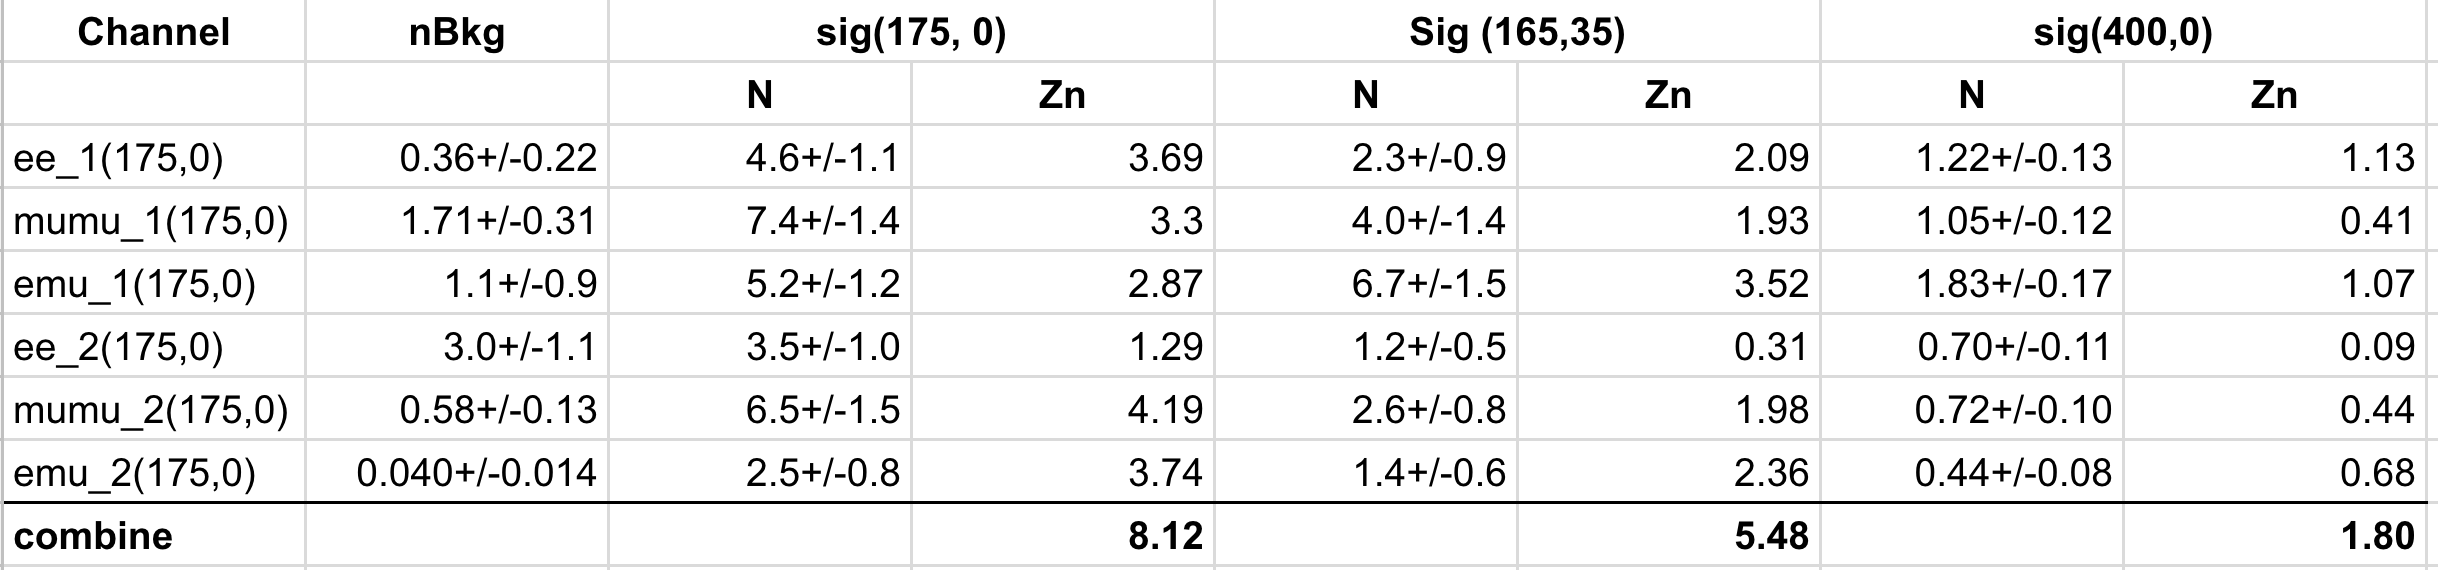
\includegraphics[width=\textwidth]{data/optimization/dongliang.png}
\end{frame}

\begin{frame}[fragile]{optimization}
\tiny
\begin{verbatim}
SR_SS_ee_1_opt: (175, 0):
45 <= pt1 < -1
20 <= pt2 < -1
0 <= ptll < -1
70 <= mTtwo < -1
0 <= fabs(eta1-eta2) < -1
55 <= METRel < -1
280 <= meff < 430
135 <= mtm < -1
0 <= mlj < 90

Zjets: 0 +/- 0 (0)
Wjets: 0 +/- 0 (0)
top: 0 +/- 0 (0)
VV: -0.0121278 +/- 0.280146 (50)
Vgamma: 0 +/- 0 (0)
VVV: 6.26348e-05 +/- 6.26348e-05 (1)
Higgs: 0 +/- 0 (0)
Total BG: 6.26348e-05 +/- 6.26348e-05 (51)

Signal (175, 0): 1.39928 +/- 0.582325 (6), Significance: 4.71305
Signal (165, 35): 0 +/- 0 (0), Significance: -3.26392
Signal (400, 0): 0.558645 +/- 0.0989239 (46), Significance: 2.55986
\end{verbatim}
\end{frame}

\begin{frame}[fragile]{optimization}
\tiny
\begin{verbatim}
SR_SS_mumu_1_opt: (175, 0):
30 <= pt1 < -1
20 <= pt2 < -1
0 <= ptll < -1
95 <= mTtwo < 110
0 <= fabs(eta1-eta2) < 1.5
90 <= METRel < -1
200 <= meff < -1
140 <= mtm < -1
0 <= mlj < 90

Zjets: 0 +/- 0 (0)
Wjets: 0 +/- 0 (0)
top: 0 +/- 0 (0)
VV: -0.0682857 +/- 0.118165 (15)
Vgamma: 0 +/- 0 (0)
VVV: 0.000545925 +/- 0.000545925 (1)
Higgs: 0 +/- 0 (0)
Total BG: 0.000545925 +/- 0.000545925 (16)

Signal (175, 0): 1.96123 +/- 0.765857 (7), Significance: 5.01703
Signal (165, 35): 0 +/- 0 (0), Significance: -2.67333
Signal (400, 0): 0.124436 +/- 0.0389975 (11), Significance: 0.207614
\end{verbatim}
\end{frame}

\begin{frame}[fragile]{optimization}
\tiny
\begin{verbatim}
SR_SS_emu_1_opt: (175, 0):
30 <= pt1 < -1
35 <= pt2 < -1
0 <= ptll < 120
95 <= mTtwo < -1
0 <= fabs(eta1-eta2) < -1
75 <= METRel < -1
230 <= meff < -1
70 <= mtm < -1
0 <= mlj < 90

Zjets: 0 +/- 0 (0)
Wjets: 0 +/- 0 (0)
top: 0.00927442 +/- 0.00985018 (5)
VV: -0.442302 +/- 0.637069 (32)
Vgamma: 0 +/- 0 (0)
VVV: 0.018226 +/- 0.0111345 (4)
Higgs: 0 +/- 0 (0)
Total BG: 0.0275004 +/- 0.0148661 (41)

Signal (175, 0): 4.86875 +/- 2.15685 (14), Significance: 6.06079
Signal (165, 35): 1.31551 +/- 0.543934 (6), Significance: 2.43184
Signal (400, 0): 0.398847 +/- 0.0677367 (37), Significance: 0.680404
\end{verbatim}
\end{frame}

\begin{frame}[fragile]{optimization}
\tiny
\begin{verbatim}
SR_SS_ee_2_opt: (175, 0):
30 <= pt1 < -1
20 <= pt2 < -1
0 <= ptll < -1
85 <= mTtwo < 100
0 <= fabs(eta1-eta2) < -1
10 <= METRel < -1
240 <= meff < 370
110 <= mtm < -1
0 <= mlj < 120

Zjets: 0 +/- 0 (0)
Wjets: 0 +/- 0 (0)
top: 0.00365115 +/- 0.0100206 (6)
VV: -0.0432296 +/- 0.112286 (18)
Vgamma: 0 +/- 0 (0)
VVV: 0 +/- 0 (0)
Higgs: 0.00259053 +/- 0.00185347 (2)
Total BG: 0.00624168 +/- 0.0101906 (26)

Signal (175, 0): 2.03314 +/- 0.834362 (7), Significance: 4.10945
Signal (165, 35): 0 +/- 0 (0), Significance: -1.91897
Signal (400, 0): 0.0177716 +/- 0.0125684 (2), Significance: -1.27025
\end{verbatim}
\end{frame}

\begin{frame}[fragile]{optimization}
\tiny
\begin{verbatim}
SR_SS_mumu_2_opt: (175, 0):
50 <= pt1 < -1
30 <= pt2 < -1
60 <= ptll < -1
70 <= mTtwo < -1
0 <= fabs(eta1-eta2) < 1.5
0 <= METRel < -1
200 <= meff < -1
75 <= mtm < -1
0 <= mlj < 120

Zjets: 0 +/- 0 (0)
Wjets: 0 +/- 0 (0)
top: 0.0155577 +/- 0.0116699 (11)
VV: 0.472923 +/- 0.116725 (126)
Vgamma: 0 +/- 0 (0)
VVV: 0.0932022 +/- 0.0559424 (5)
Higgs: 0.00298778 +/- 0.00454967 (6)
Total BG: 0.58467 +/- 0.130043 (148)

Signal (175, 0): 6.47802 +/- 1.50372 (22), Significance: 4.18942
Signal (165, 35): 2.57524 +/- 0.822315 (10), Significance: 1.9832
Signal (400, 0): 0.720309 +/- 0.102326 (59), Significance: 0.43552
\end{verbatim}
\end{frame}

\begin{frame}[fragile]{optimization}
\tiny
\begin{verbatim}
SR_SS_emu_2_opt: (175, 0):
30 <= pt1 < -1
25 <= pt2 < -1
0 <= ptll < -1
65 <= mTtwo < -1
0 <= fabs(eta1-eta2) < 2
85 <= METRel < -1
200 <= meff < -1
160 <= mtm < 215
0 <= mlj < 120

Zjets: 0 +/- 0 (0)
Wjets: -0.0546401 +/- 0.0546401 (1)
top: 0.0091173 +/- 0.00862592 (8)
VV: -0.0114641 +/- 0.0777707 (32)
Vgamma: 0 +/- 0 (0)
VVV: 0 +/- 0 (0)
Higgs: 0.00476373 +/- 0.00333049 (5)
Total BG: 0.013881 +/- 0.00924655 (46)

Signal (175, 0): 2.94275 +/- 0.842809 (13), Significance: 4.77428
Signal (165, 35): 1.40231 +/- 0.575725 (6), Significance: 2.85739
Signal (400, 0): 0.477849 +/- 0.0808605 (43), Significance: 1.07351
\end{verbatim}
\end{frame}

\section{Conclusion}
\begin{frame}{Conclusion}
\begin{itemize}
\item Conclusion:
\begin{itemize}
\item We should see significant excess if the signal exist
\item We can exclude the signal if they are not exist
\end{itemize}
\item Few issues need to further study:
\begin{itemize}
\item The global maximum for significance is difficult to find.
\item The low statistics of background sample.
\item need to understand some of the optimization results.
\end{itemize}
\end{itemize}
\end{frame}

\section{Plan}
\begin{frame}{Plan}
\begin{itemize}
\item Dani and Samuel will agree on the SR selection (compare and agree on the final signal selection cuts).
\item Dongliang and Samuel will work on data/MC plots after pre-selection level (all lepton cuts, possibly also jets and b-jets cuts).
\item Plot the electron eta to make a decision about whether we use the electrons in the crack region.
\item Estimate charge flip BG and fake BG from data, both in SR and pre-selection level.
\end{itemize}
\end{frame}

\begin{frame}
\begin{center}
\huge
Backup
\end{center}
\end{frame}

\begin{frame}{Selection in run1 SR}
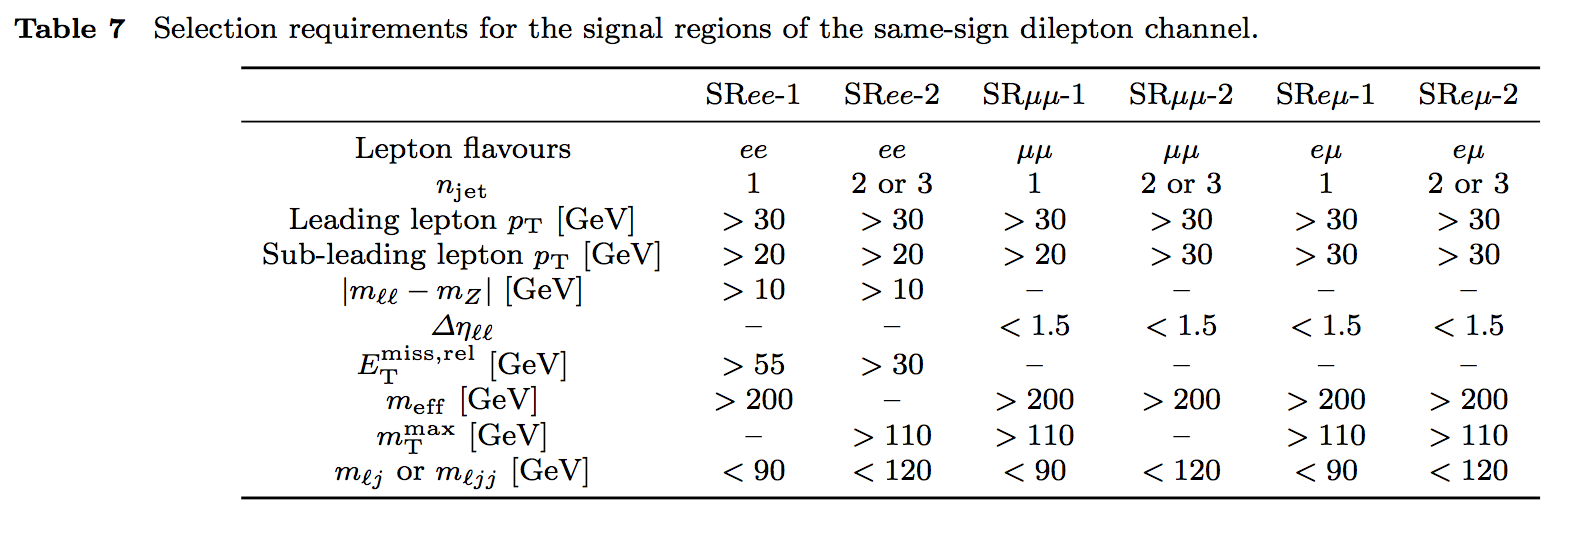
\includegraphics[width=\textwidth]{data/photo/SRcutrun1.png} \\
\url{https://arxiv.org/pdf/1501.07110.pdf}
\end{frame}

\begin{frame}
\frametitle{significance calculation}
\begin{itemize}
\item RooStats::NumberCountingUtils::BinomialExpZ(S,B,$\delta$B)
\item $\delta$B = 0.3
\end{itemize}
\end{frame}

\begin{frame}[fragile]{pre-selection}
\tiny
\begin{verbatim}
SR_SS_ee_1:
nCJet == 1
nBJet == 0
fabs(mll - 91.2) > 10

SR_SS_mumu_1:
nCJet == 1
nBJet == 0
fabs(eta1) < 2.4
fabs(eta2) < 2.4

SR_SS_emu_1:
nCJet == 1
nBJet == 0
fabs(eta1) < 2.5
fabs(eta2) < 2.5

SR_SS_ee_2:
nCJet == 2 || nCJet == 3
nBJet == 0
fabs(mll - 91.2) > 10

SR_SS_mumu_2:
nCJet == 2 || nCJet == 3
nBJet == 0
fabs(eta1) < 2.4
fabs(eta2) < 2.4

SR_SS_emu_2:
nCJet == 2 || nCJet == 3
nBJet == 0
fabs(eta1) < 2.5
fabs(eta2) < 2.5
\end{verbatim}
\end{frame}

\begin{frame}[fragile]{optimization}
\tiny
\begin{verbatim}
SR_SS_ee_1_opt: (175, 0):
45 <= pt1
20 <= pt2
0 <= ptll
70 <= mTtwo
0 <= fabs(eta1-eta2)
55 <= METRel
280 <= meff < 430
135 <= mtm
0 <= mlj < 90

Zjets: 0 +/- 0 (0)
Wjets: 0 +/- 0 (0)
top: 0 +/- 0 (0)
VV: -0.0121278 +/- 0.280146 (50)
Vgamma: 0 +/- 0 (0)
VVV: 6.26348e-05 +/- 6.26348e-05 (1)
Higgs: 0 +/- 0 (0)
Total BG: 6.26348e-05 +/- 6.26348e-05 (51)

Signal (175, 0): 1.39928 +/- 0.582325 (6), Significance: 4.71305
Signal (165, 35): 0 +/- 0 (0), Significance: -3.26392
Signal (400, 0): 0.558645 +/- 0.0989239 (46), Significance: 2.55986
\end{verbatim}
\end{frame}

\begin{frame}[fragile]{optimization}
\tiny
\begin{verbatim}
SR_SS_mumu_1_opt: (175, 0):
30 <= pt1
20 <= pt2
0 <= ptll
95 <= mTtwo < 110
0 <= fabs(eta1-eta2) < 1.5
90 <= METRel
200 <= meff
140 <= mtm
0 <= mlj < 90

Zjets: 0 +/- 0 (0)
Wjets: 0 +/- 0 (0)
top: 0 +/- 0 (0)
VV: -0.0682857 +/- 0.118165 (15)
Vgamma: 0 +/- 0 (0)
VVV: 0.000545925 +/- 0.000545925 (1)
Higgs: 0 +/- 0 (0)
Total BG: 0.000545925 +/- 0.000545925 (16)

Signal (175, 0): 1.96123 +/- 0.765857 (7), Significance: 5.01703
Signal (165, 35): 0 +/- 0 (0), Significance: -2.67333
Signal (400, 0): 0.124436 +/- 0.0389975 (11), Significance: 0.207614
\end{verbatim}
\end{frame}

\begin{frame}[fragile]{optimization}
\tiny
\begin{verbatim}
SR_SS_emu_1_opt: (175, 0):
30 <= pt1
35 <= pt2
0 <= ptll < 120
95 <= mTtwo
0 <= fabs(eta1-eta2)
75 <= METRel
230 <= meff
70 <= mtm
0 <= mlj < 90

Zjets: 0 +/- 0 (0)
Wjets: 0 +/- 0 (0)
top: 0.00927442 +/- 0.00985018 (5)
VV: -0.442302 +/- 0.637069 (32)
Vgamma: 0 +/- 0 (0)
VVV: 0.018226 +/- 0.0111345 (4)
Higgs: 0 +/- 0 (0)
Total BG: 0.0275004 +/- 0.0148661 (41)

Signal (175, 0): 4.86875 +/- 2.15685 (14), Significance: 6.06079
Signal (165, 35): 1.31551 +/- 0.543934 (6), Significance: 2.43184
Signal (400, 0): 0.398847 +/- 0.0677367 (37), Significance: 0.680404
\end{verbatim}
\end{frame}

\begin{frame}[fragile]{optimization}
\tiny
\begin{verbatim}
SR_SS_ee_2_opt: (175, 0):
30 <= pt1
20 <= pt2
0 <= ptll
85 <= mTtwo < 100
0 <= fabs(eta1-eta2)
10 <= METRel
240 <= meff < 370
110 <= mtm
0 <= mlj < 120

Zjets: 0 +/- 0 (0)
Wjets: 0 +/- 0 (0)
top: 0.00365115 +/- 0.0100206 (6)
VV: -0.0432296 +/- 0.112286 (18)
Vgamma: 0 +/- 0 (0)
VVV: 0 +/- 0 (0)
Higgs: 0.00259053 +/- 0.00185347 (2)
Total BG: 0.00624168 +/- 0.0101906 (26)

Signal (175, 0): 2.03314 +/- 0.834362 (7), Significance: 4.10945
Signal (165, 35): 0 +/- 0 (0), Significance: -1.91897
Signal (400, 0): 0.0177716 +/- 0.0125684 (2), Significance: -1.27025
\end{verbatim}
\end{frame}

\begin{frame}[fragile]{optimization}
\tiny
\begin{verbatim}
SR_SS_mumu_2_opt: (175, 0):
50 <= pt1
30 <= pt2
60 <= ptll
70 <= mTtwo
0 <= fabs(eta1-eta2) < 1.5
0 <= METRel
200 <= meff
75 <= mtm
0 <= mlj < 120

Zjets: 0 +/- 0 (0)
Wjets: 0 +/- 0 (0)
top: 0.0155577 +/- 0.0116699 (11)
VV: 0.472923 +/- 0.116725 (126)
Vgamma: 0 +/- 0 (0)
VVV: 0.0932022 +/- 0.0559424 (5)
Higgs: 0.00298778 +/- 0.00454967 (6)
Total BG: 0.58467 +/- 0.130043 (148)

Signal (175, 0): 6.47802 +/- 1.50372 (22), Significance: 4.18942
Signal (165, 35): 2.57524 +/- 0.822315 (10), Significance: 1.9832
Signal (400, 0): 0.720309 +/- 0.102326 (59), Significance: 0.43552
\end{verbatim}
\end{frame}

\begin{frame}[fragile]{optimization}
\tiny
\begin{verbatim}
SR_SS_emu_2_opt: (175, 0):
30 <= pt1
25 <= pt2
0 <= ptll
65 <= mTtwo
0 <= fabs(eta1-eta2) < 2
85 <= METRel
200 <= meff
160 <= mtm < 215
0 <= mlj < 120

Zjets: 0 +/- 0 (0)
Wjets: -0.0546401 +/- 0.0546401 (1)
top: 0.0091173 +/- 0.00862592 (8)
VV: -0.0114641 +/- 0.0777707 (32)
Vgamma: 0 +/- 0 (0)
VVV: 0 +/- 0 (0)
Higgs: 0.00476373 +/- 0.00333049 (5)
Total BG: 0.013881 +/- 0.00924655 (46)

Signal (175, 0): 2.94275 +/- 0.842809 (13), Significance: 4.77428
Signal (165, 35): 1.40231 +/- 0.575725 (6), Significance: 2.85739
Signal (400, 0): 0.477849 +/- 0.0808605 (43), Significance: 1.07351

\end{verbatim}
\end{frame}

\begin{frame}[fragile]{optimization}
\tiny
\begin{verbatim}
SR_SS_ee_1_opt: (165, 35):
40 <= pt1
20 <= pt2
0 <= ptll
55 <= mTtwo
0 <= fabs(eta1-eta2)
60 <= METRel
200 <= meff
125 <= mtm < 150
0 <= mlj < 90

Zjets: 0 +/- 0 (0)
Wjets: 0 +/- 0 (0)
top: 0.0181436 +/- 0.0080057 (6)
VV: -0.78323 +/- 1.06585 (88)
Vgamma: 0 +/- 0 (0)
VVV: 0.0111816 +/- 0.00906818 (2)
Higgs: -0.00010123 +/- 0.00192543 (2)
Total BG: 0.0293251 +/- 0.0120964 (98)

Signal (175, 0): 2.18556 +/- 0.698057 (10), Significance: 3.52133
Signal (165, 35): 2.42605 +/- 0.890616 (8), Significance: 3.78992
Signal (400, 0): 0.139056 +/- 0.0721997 (7), Significance: -0.247445
\end{verbatim}
\end{frame}

\begin{frame}[fragile]{optimization}
\tiny
\begin{verbatim}
SR_SS_mumu_1_opt: (165, 35):
50 <= pt1
20 <= pt2
0 <= ptll
0 <= mTtwo
0 <= fabs(eta1-eta2) < 1
0 <= METRel
200 <= meff
100 <= mtm
0 <= mlj < 90

Zjets: 0 +/- 0 (0)
Wjets: 0 +/- 0 (0)
top: 0.142494 +/- 0.0356254 (32)
VV: 4.02273 +/- 0.650296 (785)
Vgamma: 0 +/- 0 (0)
VVV: 0.218855 +/- 0.0517602 (28)
Higgs: 0.389218 +/- 0.37774 (4)
Total BG: 4.7733 +/- 0.754665 (849)

Signal (175, 0): 12.3469 +/- 1.93532 (49), Significance: 3.18249
Signal (165, 35): 12.0307 +/- 2.30876 (34), Significance: 3.11525
Signal (400, 0): 1.07591 +/- 0.132611 (84), Significance: 0.168546
\end{verbatim}
\end{frame}

\begin{frame}[fragile]{optimization}
\tiny
\begin{verbatim}
SR_SS_emu_1_opt: (165, 35):
30 <= pt1
30 <= pt2
0 <= ptll
75 <= mTtwo < 85
0 <= fabs(eta1-eta2) < 1.5
0 <= METRel
200 <= meff
145 <= mtm < 180
0 <= mlj < 90

Zjets: 0 +/- 0 (0)
Wjets: 0 +/- 0 (0)
top: 0.00439834 +/- 0.00439834 (1)
VV: -0.00992742 +/- 0.0849192 (22)
Vgamma: 0 +/- 0 (0)
VVV: 0 +/- 0 (0)
Higgs: 0 +/- 0 (0)
Total BG: 0.00439834 +/- 0.00439834 (23)

Signal (175, 0): 0 +/- 0 (0), Significance: -2.03456
Signal (165, 35): 2.37122 +/- 0.917571 (7), Significance: 4.71551
Signal (400, 0): 0 +/- 0 (0), Significance: -2.03456
\end{verbatim}
\end{frame}

\begin{frame}[fragile]{optimization}
\tiny
\begin{verbatim}
SR_SS_ee_2_opt: (165, 35):
35 <= pt1
20 <= pt2
0 <= ptll
0 <= mTtwo
0 <= fabs(eta1-eta2)
25 <= METRel
250 <= meff
130 <= mtm < 135
0 <= mlj < 120

Zjets: 0 +/- 0 (0)
Wjets: 0 +/- 0 (0)
top: 0 +/- 0 (0)
VV: 0.099032 +/- 0.098807 (43)
Vgamma: 0 +/- 0 (0)
VVV: 0.0109896 +/- 0.0109896 (1)
Higgs: 0 +/- 0 (0)
Total BG: 0.110022 +/- 0.0994162 (44)

Signal (175, 0): 0.182675 +/- 0.182675 (1), Significance: -0.194637
Signal (165, 35): 1.40047 +/- 0.635882 (5), Significance: 1.89768
Signal (400, 0): 0.0235248 +/- 0.0166348 (2), Significance: -0.798383
\end{verbatim}
\end{frame}

\begin{frame}[fragile]{optimization}
\tiny
\begin{verbatim}
SR_SS_mumu_2_opt: (165, 35):
35 <= pt1
25 <= pt2
10 <= ptll
25 <= mTtwo
0 <= fabs(eta1-eta2) < 1.5
0 <= METRel
250 <= meff
55 <= mtm
0 <= mlj < 120

Zjets: 0 +/- 0 (0)
Wjets: 0.285912 +/- 0.224433 (2)
top: 0.167552 +/- 0.0299649 (70)
VV: 4.0527 +/- 0.564459 (1129)
Vgamma: 0 +/- 0 (0)
VVV: 0.173665 +/- 0.0748373 (12)
Higgs: 0.42397 +/- 0.393193 (19)
Total BG: 5.1038 +/- 0.728068 (1232)

Signal (175, 0): 9.94131 +/- 1.65048 (39), Significance: 2.56149
Signal (165, 35): 11.8525 +/- 1.92008 (43), Significance: 2.97414
Signal (400, 0): 1.14455 +/- 0.125258 (96), Significance: 0.178149
\end{verbatim}
\end{frame}

\begin{frame}[fragile]{optimization}
\tiny
\begin{verbatim}
SR_SS_emu_2_opt: (165, 35):
30 <= pt1
45 <= pt2
60 <= ptll < 100
0 <= mTtwo
0 <= fabs(eta1-eta2) < 1
60 <= METRel
200 <= meff
120 <= mtm
0 <= mlj < 120

Zjets: 0 +/- 0 (0)
Wjets: 0 +/- 0 (0)
top: 0.00975607 +/- 0.00734236 (5)
VV: 0.144638 +/- 0.0610572 (51)
Vgamma: 0 +/- 0 (0)
VVV: 0.00895897 +/- 0.00868043 (2)
Higgs: 0 +/- 0 (0)
Total BG: 0.163353 +/- 0.0621067 (58)

Signal (175, 0): 1.61211 +/- 0.574098 (8), Significance: 1.93628
Signal (165, 35): 3.46066 +/- 1.12495 (11), Significance: 3.58767
Signal (400, 0): 0.0824434 +/- 0.027741 (9), Significance: -0.49963

\end{verbatim}
\end{frame}

\begin{frame}[fragile]{optimization}
\tiny
\begin{verbatim}
SR_SS_ee_1_opt: (400, 0):
70 <= pt1
20 <= pt2
70 <= ptll
80 <= mTtwo
0 <= fabs(eta1-eta2)
85 <= METRel
260 <= meff
105 <= mtm
0 <= mlj < 90

Zjets: 0 +/- 0 (0)
Wjets: 0 +/- 0 (0)
top: 0.00838462 +/- 0.00592988 (2)
VV: 0.0523514 +/- 0.30376 (50)
Vgamma: 0.0525887 +/- 0.0372236 (2)
VVV: 0.0164977 +/- 0.00996812 (5)
Higgs: 0 +/- 0 (0)
Total BG: 0.129822 +/- 0.306252 (59)

Signal (175, 0): 0.910416 +/- 0.461477 (4), Significance: 1.17902
Signal (165, 35): 0.253865 +/- 0.253865 (1), Significance: -0.0152519
Signal (400, 0): 1.03059 +/- 0.12497 (87), Significance: 1.3471
\end{verbatim}
\end{frame}

\begin{frame}[fragile]{optimization}
\tiny
\begin{verbatim}
SR_SS_mumu_1_opt: (400, 0):
30 <= pt1
20 <= pt2
0 <= ptll
90 <= mTtwo
0 <= fabs(eta1-eta2)
5 <= METRel
250 <= meff
165 <= mtm
0 <= mlj < 90

Zjets: 0 +/- 0 (0)
Wjets: 0 +/- 0 (0)
top: 0.00685964 +/- 0.00486751 (2)
VV: 0.155216 +/- 0.140061 (31)
Vgamma: 0 +/- 0 (0)
VVV: 0.0314002 +/- 0.0187823 (5)
Higgs: 0 +/- 0 (0)
Total BG: 0.193476 +/- 0.141399 (38)

Signal (175, 0): 1.56757 +/- 0.863777 (4), Significance: 1.79857
Signal (165, 35): 0 +/- 0 (0), Significance: -0.749027
Signal (400, 0): 1.01371 +/- 0.133711 (78), Significance: 1.15897
\end{verbatim}
\end{frame}

\begin{frame}[fragile]{optimization}
\tiny
\begin{verbatim}
SR_SS_emu_1_opt: (400, 0):
35 <= pt1
30 <= pt2
0 <= ptll
100 <= mTtwo
0 <= fabs(eta1-eta2)
95 <= METRel
200 <= meff
125 <= mtm
0 <= mlj < 90

Zjets: 0.0150102 +/- 0.0150102 (1)
Wjets: 0 +/- 0 (0)
top: 0.01401 +/- 0.00888758 (5)
VV: 0.00322195 +/- 0.647186 (55)
Vgamma: 0.0513547 +/- 0.0324214 (3)
VVV: 0.0394613 +/- 0.0186369 (6)
Higgs: 0.00258108 +/- 0.00258108 (1)
Total BG: 0.125639 +/- 0.648506 (71)

Signal (175, 0): 2.17543 +/- 0.664132 (11), Significance: 2.66428
Signal (165, 35): 1.15292 +/- 0.594712 (4), Significance: 1.52405
Signal (400, 0): 1.74154 +/- 0.161934 (147), Significance: 2.21878
\end{verbatim}
\end{frame}

\begin{frame}[fragile]{optimization}
\tiny
\begin{verbatim}
SR_SS_ee_2_opt: (400, 0):
30 <= pt1
20 <= pt2
0 <= ptll
0 <= mTtwo
0 <= fabs(eta1-eta2)
30 <= METRel
0 <= meff
110 <= mtm
0 <= mlj < 120

Zjets: 1.86673 +/- 2.00713 (3)
Wjets: 0.385801 +/- 0.4468 (7)
top: 1.12277 +/- 0.554989 (47)
VV: 6.13975 +/- 2.55588 (614)
Vgamma: 1.35479 +/- 0.737673 (8)
VVV: 0.105014 +/- 0.0404224 (16)
Higgs: 0.526728 +/- 0.515058 (15)
Total BG: 11.5016 +/- 3.44671 (710)

Signal (175, 0): 5.02234 +/- 1.16344 (21), Significance: 0.74716
Signal (165, 35): 4.23108 +/- 1.07097 (16), Significance: 0.607607
Signal (400, 0): 0.833553 +/- 0.117127 (66), Significance: -0.0384218
\end{verbatim}
\end{frame}

\begin{frame}[fragile]{optimization}
\tiny
\begin{verbatim}
SR_SS_mumu_2_opt: (400, 0):
30 <= pt1
25 <= pt2
0 <= ptll
0 <= mTtwo
0 <= fabs(eta1-eta2)
25 <= METRel
360 <= meff
175 <= mtm
0 <= mlj < 120

Zjets: 0 +/- 0 (0)
Wjets: 0 +/- 0 (0)
top: 0.0148443 +/- 0.00888632 (6)
VV: 0.550109 +/- 0.10186 (121)
Vgamma: 0 +/- 0 (0)
VVV: 0.0842916 +/- 0.0554874 (4)
Higgs: 0.00105538 +/- 0.00105538 (1)
Total BG: 0.6503 +/- 0.116338 (132)

Signal (175, 0): 1.94164 +/- 0.714345 (8), Significance: 1.45837
Signal (165, 35): 1.02242 +/- 0.51558 (4), Significance: 0.699564
Signal (400, 0): 1.0043 +/- 0.117149 (85), Significance: 0.682855
\end{verbatim}
\end{frame}

\begin{frame}[fragile]{optimization}
\tiny
\begin{verbatim}
SR_SS_emu_2_opt: (400, 0):
25 <= pt1
30 <= pt2
0 <= ptll
80 <= mTtwo
0 <= fabs(eta1-eta2)
5 <= METRel
330 <= meff
170 <= mtm
0 <= mlj < 120

Zjets: 0 +/- 0 (0)
Wjets: 0 +/- 0 (0)
top: 0.00478847 +/- 0.00560986 (4)
VV: -0.0204046 +/- 0.0724784 (20)
Vgamma: 0 +/- 0 (0)
VVV: 0.0189209 +/- 0.0120301 (3)
Higgs: 0.000146774 +/- 0.00186469 (2)
Total BG: 0.0238562 +/- 0.0134041 (29)

Signal (175, 0): 1.1307 +/- 0.508417 (5), Significance: 2.20734
Signal (165, 35): 0.205295 +/- 0.205295 (1), Significance: 0.0755819
Signal (400, 0): 1.09575 +/- 0.115698 (101), Significance: 2.15059
\end{verbatim}
\end{frame}


\begin{frame}[fragile]
\frametitle{Signal sample}
\small
Sample Name(p2972 tag):
\tiny
\begin{verbatim}
mc15_13TeV.993820.MGPy8EG_A14N13LO_C1N2_Wh_2L_175_0.merge.DAOD_SUSY2.e5678_a766_a821_r7676_p2949_p2972
mc15_13TeV.993821.MGPy8EG_A14N13LO_C1N2_Wh_2L_165_35.merge.DAOD_SUSY2.e5678_a766_a821_r7676_p2949_p2972
mc15_13TeV.993822.MGPy8EG_A14N13LO_C1N2_Wh_2L_400_0.merge.DAOD_SUSY2.e5678_a766_a821_r7676_p2949_p2972
\end{verbatim}
\end{frame}

\begin{frame}[fragile]
\frametitle{Data}
\small
use both 2015 and 2016 data (3212.96 + 32861.6) /pb
\tiny
\begin{verbatim}
GRL:
GoodRunsLists/data16_13TeV/20161101/physics_25ns_20.7.xml
GoodRunsLists/data15_13TeV/20160720/physics_25ns_20.7.xml
\end{verbatim}
\end{frame}

\begin{frame}{MC BG}
p-tag: p2949
\end{frame}

\begin{frame}[fragile]
\small
Trigger list:\\
\scriptsize
\begin{verbatim}
2015
HLT_2e12_lhloose_L12EM10VH
HLT_e17_lhloose_mu14
HLT_mu18_mu8noL1

2016(A-D3)
HLT_2e17_lhvloose_nod0
HLT_e17_lhloose_nod0_mu14
HLT_mu20_mu8noL1

2016(D3-)
HLT_2e17_lhvloose_nod0
HLT_e17_lhloose_nod0_mu14
HLT_mu22_mu8noL1
\end{verbatim}
\end{frame}

\begin{frame}{Object Definitions}
\small
Tool: AnalysisBase 2.4.31, SUSYTools-00-08-60\\

\centering
\begin{table}
\small
\begin{tabularx}{\textwidth}{p{1.5cm} | p{3cm} | p{3cm} | p{3cm}}
& \textbf{Electron} & \textbf{Muon} & \textbf{Jet}\\
\hline
\textbf{Baseline}
& - $p_T>10$ GeV \newline - $|\eta^{cluster}| < 2.47$ \newline - LooseAndBLayerLLH
& - $p_T>10$ GeV \newline - $|\eta| < 2.7$ \newline - Medium
& - $p_T>20$ GeV \\
\hline
\textbf{Signal}
& - $p_T > 25$ GeV \newline - $|\eta^{cluster}| < 2.47$ \newline - TightLLH \newline - GradientLoose \newline - $|z_0 \sin \theta| < 0.5$mm \newline - $|d_0/\sigma_{d_0}| < 5$
& - $p_T > 25$ GeV \newline - $|\eta| < 2.7$ \newline - Medium \newline - GradientLoose \newline - $|z_0 \sin \theta| < 0.5$mm \newline - $|d_0/\sigma_{d_0}| < 3$
& - $p_T > 20$ GeV \newline - $|\eta|<2.8$ \newline \newline - $|JVT| > 0.59$ \newline if $p_T < 60$ GeV \newline and $|\eta| < 2.4$
\end{tabularx}
\end{table}

\raggedright
Selection:
\begin{itemize}
%\item Trigger selection
\item Exactly 2 baseline leptons and exactly 2 signal leptons
\end{itemize}

\tiny
Note: \\
Pileup reweighting is applied. \\
Scale factor for reconstruction, isolation, ID and trigger is applied.
\end{frame}

\begin{frame}
\frametitle{Definition of jets}
\normalsize
\begin{itemize}
\item Central jets: $\pt>20$ GeV, $|\eta|<2.4$, no b-tagged
\item B-jets: b-tagged
\end{itemize}
\end{frame}

\begin{frame}
\frametitle{definition of variables}
\normalsize
\begin{itemize}
\item HT: Sum of the $p_T$ of all signal jets and the two leptons.
\item R2 = MET / (MET + pt1 + pt2)
\item l12\_dPhi: difference in phi between the two leptons.
\item l12\_MET\_dPhi: difference in phi between MET and the sum of 4-momentum of the two leptons.
\end{itemize}
\end{frame}

%\begin{frame}{Expected number of events \\ For SR\_SS\_ee\_1}
\vspace{5mm}
\begin{tabular}{|c|c|c|}
\hline
& Number of events & Significance \\
\hline
Z+jets & $18.9\pm19.8$ & \\
\hline
W+jets & $3.3\pm2.1$ & \\
\hline
top & $69.1\pm5.8$ & \\
\hline
VV & $14.1\pm2.0$ & \\
\hline
V$+\gamma$ & $12.2\pm5.5$ & \\
\hline
VVV & $0.4\pm0.1$ & \\
\hline
Total BG & $117.9\pm21.6$ & \\
\hline
Signal (175, 0) & $7.1\pm1.2$ &$-0.009$\\
\hline
Signal (165, 35) & $2.4\pm0.4$ &$-0.134$\\
\hline
Signal (400, 0) & $9.8\pm0.8$ &$0.062$\\
\hline

\end{tabular}
\end{frame}

\begin{frame}{Expected number of events \\ For SR\_SS\_mumu\_1}
\vspace{5mm}
\begin{tabular}{|c|c|c|}
\hline
& Number of events & Significance \\
\hline
Z+jets & $6.4\pm6.5$ & \\
\hline
W+jets & $0.4\pm0.4$ & \\
\hline
top & $4.0\pm0.8$ & \\
\hline
VV & $7.1\pm0.7$ & \\
\hline
V$+\gamma$ & $0.0\pm0.0$ & \\
\hline
VVV & $0.3\pm0.1$ & \\
\hline
Total BG & $18.3\pm6.6$ & \\
\hline
Signal (175, 0) & $5.4\pm0.8$ &$0.531$\\
\hline
Signal (165, 35) & $2.6\pm0.5$ &$0.159$\\
\hline
Signal (400, 0) & $9.0\pm0.9$ &$0.960$\\
\hline

\end{tabular}
\end{frame}

\begin{frame}{Expected number of events \\ For SR\_SS\_emu\_1}
\vspace{5mm}
\begin{tabular}{|c|c|c|}
\hline
& Number of events & Significance \\
\hline
Z+jets & $0.1\pm0.0$ & \\
\hline
W+jets & $5.0\pm2.4$ & \\
\hline
top & $39.9\pm3.6$ & \\
\hline
VV & $14.9\pm1.8$ & \\
\hline
V$+\gamma$ & $1.5\pm0.5$ & \\
\hline
VVV & $0.4\pm0.1$ & \\
\hline
Total BG & $61.9\pm4.7$ & \\
\hline
Signal (175, 0) & $8.1\pm1.2$ &$0.191$\\
\hline
Signal (165, 35) & $5.5\pm0.6$ &$0.068$\\
\hline
Signal (400, 0) & $15.0\pm1.1$ &$0.501$\\
\hline

\end{tabular}
\end{frame}

\begin{frame}{Expected number of events \\ For SR\_SS\_ee\_2}
\vspace{5mm}
\begin{tabular}{|c|c|c|}
\hline
& Number of events & Significance \\
\hline
VV & $2.8\pm0.4$ & \\
\hline
V$+\gamma$ & $2.3\pm1.2$ & \\
\hline
Total BG & $5.1\pm1.2$ & \\
\hline
Signal (400, 380) & $0.0\pm0.0$ &$-0.229$\\
\hline
Signal (500, 450) & $0.1\pm0.0$ &$-0.188$\\
\hline
Signal (400, 300) & $0.8\pm0.1$ &$0.045$\\
\hline
Signal (400, 200) & $0.5\pm0.1$ &$-0.040$\\
\hline
Signal (400, 100) & $0.4\pm0.2$ &$-0.088$\\
\hline

\end{tabular}
\end{frame}

\begin{frame}{Expected number of events \\ For SR\_SS\_mumu\_2}
\vspace{5mm}
\begin{tabular}{|c|c|c|}
\hline
& Number of events & Significance \\
\hline
Z+jets & $89.3\pm27.3$ & \\
\hline
W+jets & $1.1\pm0.6$ & \\
\hline
top & $10.7\pm1.5$ & \\
\hline
VV & $16.3\pm0.7$ & \\
\hline
V$+\gamma$ & $2.5\pm1.3$ & \\
\hline
VVV & $0.3\pm0.1$ & \\
\hline
Total BG & $120.1\pm27.4$ & \\
\hline
Signal (175, 0) & $9.7\pm1.3$ &$0.055$\\
\hline
Signal (165, 35) & $4.1\pm0.5$ &$-0.091$\\
\hline
Signal (400, 0) & $7.5\pm0.7$ &$-0.003$\\
\hline

\end{tabular}
\end{frame}

\begin{frame}{Expected number of events \\ For SR\_SS\_emu\_2}
\vspace{5mm}
\begin{tabular}{|c|c|c|}
\hline
& Number of events & Significance \\
\hline
VV & $6.0\pm0.4$ & \\
\hline
V$+\gamma$ & $1.1\pm0.8$ & \\
\hline
Total BG & $7.1\pm0.9$ & \\
\hline
Signal (400, 380) & $0.0\pm0.0$ &$-0.213$\\
\hline
Signal (500, 450) & $0.2\pm0.0$ &$-0.162$\\
\hline
Signal (400, 300) & $1.3\pm0.2$ &$0.163$\\
\hline
Signal (400, 200) & $0.8\pm0.1$ &$0.014$\\
\hline
Signal (400, 100) & $0.5\pm0.2$ &$-0.075$\\
\hline

\end{tabular}
\end{frame}


%\begin{frame}{For SR\_SS\_run1 \\ $\pt$ of the leading lepton}
\Wider[5em]{
\includegraphics[width=0.33\textwidth]{pt1_SR_SS_ee_1}
\includegraphics[width=0.33\textwidth]{pt1_SR_SS_mumu_1}
\includegraphics[width=0.33\textwidth]{pt1_SR_SS_emu_1} \\
\includegraphics[width=0.33\textwidth]{pt1_SR_SS_ee_2}
\includegraphics[width=0.33\textwidth]{pt1_SR_SS_mumu_2}
\includegraphics[width=0.33\textwidth]{pt1_SR_SS_emu_2}
}
\end{frame}

\begin{frame}{For SR\_SS\_run1 \\ $\pt$ of the subleading lepton}
\Wider[5em]{
\includegraphics[width=0.33\textwidth]{pt2_SR_SS_ee_1}
\includegraphics[width=0.33\textwidth]{pt2_SR_SS_mumu_1}
\includegraphics[width=0.33\textwidth]{pt2_SR_SS_emu_1} \\
\includegraphics[width=0.33\textwidth]{pt2_SR_SS_ee_2}
\includegraphics[width=0.33\textwidth]{pt2_SR_SS_mumu_2}
\includegraphics[width=0.33\textwidth]{pt2_SR_SS_emu_2}
}
\end{frame}

\begin{frame}{For SR\_SS\_run1 \\ $\eta$ of the leading lepton}
\Wider[5em]{
\includegraphics[width=0.33\textwidth]{eta1_SR_SS_ee_1}
\includegraphics[width=0.33\textwidth]{eta1_SR_SS_mumu_1}
\includegraphics[width=0.33\textwidth]{eta1_SR_SS_emu_1} \\
\includegraphics[width=0.33\textwidth]{eta1_SR_SS_ee_2}
\includegraphics[width=0.33\textwidth]{eta1_SR_SS_mumu_2}
\includegraphics[width=0.33\textwidth]{eta1_SR_SS_emu_2}
}
\end{frame}

\begin{frame}{For SR\_SS\_run1 \\ $\eta$ of the subleading lepton}
\Wider[5em]{
\includegraphics[width=0.33\textwidth]{eta2_SR_SS_ee_1}
\includegraphics[width=0.33\textwidth]{eta2_SR_SS_mumu_1}
\includegraphics[width=0.33\textwidth]{eta2_SR_SS_emu_1} \\
\includegraphics[width=0.33\textwidth]{eta2_SR_SS_ee_2}
\includegraphics[width=0.33\textwidth]{eta2_SR_SS_mumu_2}
\includegraphics[width=0.33\textwidth]{eta2_SR_SS_emu_2}
}
\end{frame}

\begin{frame}{For SR\_SS\_run1 \\ $\phi$ of the leading lepton}
\Wider[5em]{
\includegraphics[width=0.33\textwidth]{phi1_SR_SS_ee_1}
\includegraphics[width=0.33\textwidth]{phi1_SR_SS_mumu_1}
\includegraphics[width=0.33\textwidth]{phi1_SR_SS_emu_1} \\
\includegraphics[width=0.33\textwidth]{phi1_SR_SS_ee_2}
\includegraphics[width=0.33\textwidth]{phi1_SR_SS_mumu_2}
\includegraphics[width=0.33\textwidth]{phi1_SR_SS_emu_2}
}
\end{frame}

\begin{frame}{For SR\_SS\_run1 \\ $m_{ll}$}
\Wider[5em]{
\includegraphics[width=0.33\textwidth]{mll_SR_SS_ee_1}
\includegraphics[width=0.33\textwidth]{mll_SR_SS_mumu_1}
\includegraphics[width=0.33\textwidth]{mll_SR_SS_emu_1} \\
\includegraphics[width=0.33\textwidth]{mll_SR_SS_ee_2}
\includegraphics[width=0.33\textwidth]{mll_SR_SS_mumu_2}
\includegraphics[width=0.33\textwidth]{mll_SR_SS_emu_2}
}
\end{frame}

\begin{frame}{For SR\_SS\_run1 \\ Dilepton $\pt$}
\Wider[5em]{
\includegraphics[width=0.33\textwidth]{ptll_SR_SS_ee_1}
\includegraphics[width=0.33\textwidth]{ptll_SR_SS_mumu_1}
\includegraphics[width=0.33\textwidth]{ptll_SR_SS_emu_1} \\
\includegraphics[width=0.33\textwidth]{ptll_SR_SS_ee_2}
\includegraphics[width=0.33\textwidth]{ptll_SR_SS_mumu_2}
\includegraphics[width=0.33\textwidth]{ptll_SR_SS_emu_2}
}
\end{frame}

\begin{frame}{For SR\_SS\_run1 \\ $E_{\text{T}}^{\text{miss}}$}
\Wider[5em]{
\includegraphics[width=0.33\textwidth]{MET_SR_SS_ee_1}
\includegraphics[width=0.33\textwidth]{MET_SR_SS_mumu_1}
\includegraphics[width=0.33\textwidth]{MET_SR_SS_emu_1} \\
\includegraphics[width=0.33\textwidth]{MET_SR_SS_ee_2}
\includegraphics[width=0.33\textwidth]{MET_SR_SS_mumu_2}
\includegraphics[width=0.33\textwidth]{MET_SR_SS_emu_2}
}
\end{frame}

\begin{frame}{For SR\_SS\_run1 \\ $m_{T2}$}
\Wider[5em]{
\includegraphics[width=0.33\textwidth]{mTtwo_SR_SS_ee_1}
\includegraphics[width=0.33\textwidth]{mTtwo_SR_SS_mumu_1}
\includegraphics[width=0.33\textwidth]{mTtwo_SR_SS_emu_1} \\
\includegraphics[width=0.33\textwidth]{mTtwo_SR_SS_ee_2}
\includegraphics[width=0.33\textwidth]{mTtwo_SR_SS_mumu_2}
\includegraphics[width=0.33\textwidth]{mTtwo_SR_SS_emu_2}
}
\end{frame}

\begin{frame}{For SR\_SS\_run1 \\ $m_{\text{T}}$ of the leading lepton}
\Wider[5em]{
\includegraphics[width=0.33\textwidth]{mt1_SR_SS_ee_1}
\includegraphics[width=0.33\textwidth]{mt1_SR_SS_mumu_1}
\includegraphics[width=0.33\textwidth]{mt1_SR_SS_emu_1} \\
\includegraphics[width=0.33\textwidth]{mt1_SR_SS_ee_2}
\includegraphics[width=0.33\textwidth]{mt1_SR_SS_mumu_2}
\includegraphics[width=0.33\textwidth]{mt1_SR_SS_emu_2}
}
\end{frame}

\begin{frame}{For SR\_SS\_run1 \\ $m_{\text{T}}$ of the subleading lepton}
\Wider[5em]{
\includegraphics[width=0.33\textwidth]{mt2_SR_SS_ee_1}
\includegraphics[width=0.33\textwidth]{mt2_SR_SS_mumu_1}
\includegraphics[width=0.33\textwidth]{mt2_SR_SS_emu_1} \\
\includegraphics[width=0.33\textwidth]{mt2_SR_SS_ee_2}
\includegraphics[width=0.33\textwidth]{mt2_SR_SS_mumu_2}
\includegraphics[width=0.33\textwidth]{mt2_SR_SS_emu_2}
}
\end{frame}

\begin{frame}{For SR\_SS\_run1 \\ $\pt$ of the leading jet}
\Wider[5em]{
\includegraphics[width=0.33\textwidth]{jetpt_SR_SS_ee_1}
\includegraphics[width=0.33\textwidth]{jetpt_SR_SS_mumu_1}
\includegraphics[width=0.33\textwidth]{jetpt_SR_SS_emu_1} \\
\includegraphics[width=0.33\textwidth]{jetpt_SR_SS_ee_2}
\includegraphics[width=0.33\textwidth]{jetpt_SR_SS_mumu_2}
\includegraphics[width=0.33\textwidth]{jetpt_SR_SS_emu_2}
}
\end{frame}

\begin{frame}{For SR\_SS\_run1 \\ $\eta$ of the leading jet}
\Wider[5em]{
\includegraphics[width=0.33\textwidth]{jeteta_SR_SS_ee_1}
\includegraphics[width=0.33\textwidth]{jeteta_SR_SS_mumu_1}
\includegraphics[width=0.33\textwidth]{jeteta_SR_SS_emu_1} \\
\includegraphics[width=0.33\textwidth]{jeteta_SR_SS_ee_2}
\includegraphics[width=0.33\textwidth]{jeteta_SR_SS_mumu_2}
\includegraphics[width=0.33\textwidth]{jeteta_SR_SS_emu_2}
}
\end{frame}

\begin{frame}{For SR\_SS\_run1 \\ Number of jets}
\Wider[5em]{
\includegraphics[width=0.33\textwidth]{nJet_SR_SS_ee_1}
\includegraphics[width=0.33\textwidth]{nJet_SR_SS_mumu_1}
\includegraphics[width=0.33\textwidth]{nJet_SR_SS_emu_1} \\
\includegraphics[width=0.33\textwidth]{nJet_SR_SS_ee_2}
\includegraphics[width=0.33\textwidth]{nJet_SR_SS_mumu_2}
\includegraphics[width=0.33\textwidth]{nJet_SR_SS_emu_2}
}
\end{frame}

\begin{frame}{For SR\_SS\_run1 \\ Number of b-jets}
\Wider[5em]{
\includegraphics[width=0.33\textwidth]{nBJet_SR_SS_ee_1}
\includegraphics[width=0.33\textwidth]{nBJet_SR_SS_mumu_1}
\includegraphics[width=0.33\textwidth]{nBJet_SR_SS_emu_1} \\
\includegraphics[width=0.33\textwidth]{nBJet_SR_SS_ee_2}
\includegraphics[width=0.33\textwidth]{nBJet_SR_SS_mumu_2}
\includegraphics[width=0.33\textwidth]{nBJet_SR_SS_emu_2}
}
\end{frame}

\begin{frame}{For SR\_SS\_run1 \\ Number of central jets}
\Wider[5em]{
\includegraphics[width=0.33\textwidth]{nCJet_SR_SS_ee_1}
\includegraphics[width=0.33\textwidth]{nCJet_SR_SS_mumu_1}
\includegraphics[width=0.33\textwidth]{nCJet_SR_SS_emu_1} \\
\includegraphics[width=0.33\textwidth]{nCJet_SR_SS_ee_2}
\includegraphics[width=0.33\textwidth]{nCJet_SR_SS_mumu_2}
\includegraphics[width=0.33\textwidth]{nCJet_SR_SS_emu_2}
}
\end{frame}

\begin{frame}{For SR\_SS\_run1 \\ $\Delta\phi_{ll}$}
\Wider[5em]{
\includegraphics[width=0.33\textwidth]{l12_dPhi_SR_SS_ee_1}
\includegraphics[width=0.33\textwidth]{l12_dPhi_SR_SS_mumu_1}
\includegraphics[width=0.33\textwidth]{l12_dPhi_SR_SS_emu_1} \\
\includegraphics[width=0.33\textwidth]{l12_dPhi_SR_SS_ee_2}
\includegraphics[width=0.33\textwidth]{l12_dPhi_SR_SS_mumu_2}
\includegraphics[width=0.33\textwidth]{l12_dPhi_SR_SS_emu_2}
}
\end{frame}

\begin{frame}{For SR\_SS\_run1 \\ $\Delta\phi_{ll,\text{MET}}$}
\Wider[5em]{
\includegraphics[width=0.33\textwidth]{l12_MET_dPhi_SR_SS_ee_1}
\includegraphics[width=0.33\textwidth]{l12_MET_dPhi_SR_SS_mumu_1}
\includegraphics[width=0.33\textwidth]{l12_MET_dPhi_SR_SS_emu_1} \\
\includegraphics[width=0.33\textwidth]{l12_MET_dPhi_SR_SS_ee_2}
\includegraphics[width=0.33\textwidth]{l12_MET_dPhi_SR_SS_mumu_2}
\includegraphics[width=0.33\textwidth]{l12_MET_dPhi_SR_SS_emu_2}
}
\end{frame}

\begin{frame}{For SR\_SS\_run1 \\ $\Delta\phi_{\text{jet0,MET}}$}
\Wider[5em]{
\includegraphics[width=0.33\textwidth]{jets_MET_dPhi_SR_SS_ee_1}
\includegraphics[width=0.33\textwidth]{jets_MET_dPhi_SR_SS_mumu_1}
\includegraphics[width=0.33\textwidth]{jets_MET_dPhi_SR_SS_emu_1} \\
\includegraphics[width=0.33\textwidth]{jets_MET_dPhi_SR_SS_ee_2}
\includegraphics[width=0.33\textwidth]{jets_MET_dPhi_SR_SS_mumu_2}
\includegraphics[width=0.33\textwidth]{jets_MET_dPhi_SR_SS_emu_2}
}
\end{frame}

\begin{frame}{For SR\_SS\_run1 \\ $\Delta\eta_{ll}$}
\Wider[5em]{
\includegraphics[width=0.33\textwidth]{dEta_SR_SS_ee_1}
\includegraphics[width=0.33\textwidth]{dEta_SR_SS_mumu_1}
\includegraphics[width=0.33\textwidth]{dEta_SR_SS_emu_1} \\
\includegraphics[width=0.33\textwidth]{dEta_SR_SS_ee_2}
\includegraphics[width=0.33\textwidth]{dEta_SR_SS_mumu_2}
\includegraphics[width=0.33\textwidth]{dEta_SR_SS_emu_2}
}
\end{frame}

\begin{frame}{For SR\_SS\_run1 \\ $E_{\text{T}}^{\text{miss,rel}}$}
\Wider[5em]{
\includegraphics[width=0.33\textwidth]{METRel_SR_SS_ee_1}
\includegraphics[width=0.33\textwidth]{METRel_SR_SS_mumu_1}
\includegraphics[width=0.33\textwidth]{METRel_SR_SS_emu_1} \\
\includegraphics[width=0.33\textwidth]{METRel_SR_SS_ee_2}
\includegraphics[width=0.33\textwidth]{METRel_SR_SS_mumu_2}
\includegraphics[width=0.33\textwidth]{METRel_SR_SS_emu_2}
}
\end{frame}

\begin{frame}{For SR\_SS\_run1 \\ $m_{\text{eff}}$}
\Wider[5em]{
\includegraphics[width=0.33\textwidth]{meff_SR_SS_ee_1}
\includegraphics[width=0.33\textwidth]{meff_SR_SS_mumu_1}
\includegraphics[width=0.33\textwidth]{meff_SR_SS_emu_1} \\
\includegraphics[width=0.33\textwidth]{meff_SR_SS_ee_2}
\includegraphics[width=0.33\textwidth]{meff_SR_SS_mumu_2}
\includegraphics[width=0.33\textwidth]{meff_SR_SS_emu_2}
}
\end{frame}

\begin{frame}{For SR\_SS\_run1 \\ $m_{\text{T}}^{\text{max}}$}
\Wider[5em]{
\includegraphics[width=0.33\textwidth]{mtm_SR_SS_ee_1}
\includegraphics[width=0.33\textwidth]{mtm_SR_SS_mumu_1}
\includegraphics[width=0.33\textwidth]{mtm_SR_SS_emu_1} \\
\includegraphics[width=0.33\textwidth]{mtm_SR_SS_ee_2}
\includegraphics[width=0.33\textwidth]{mtm_SR_SS_mumu_2}
\includegraphics[width=0.33\textwidth]{mtm_SR_SS_emu_2}
}
\end{frame}

\begin{frame}{For SR\_SS\_run1 \\ $m_{lj}$ or $m_{ljj}$}
\Wider[5em]{
\includegraphics[width=0.33\textwidth]{mlj_SR_SS_ee_1}
\includegraphics[width=0.33\textwidth]{mlj_SR_SS_mumu_1}
\includegraphics[width=0.33\textwidth]{mlj_SR_SS_emu_1} \\
\includegraphics[width=0.33\textwidth]{mlj_SR_SS_ee_2}
\includegraphics[width=0.33\textwidth]{mlj_SR_SS_mumu_2}
\includegraphics[width=0.33\textwidth]{mlj_SR_SS_emu_2}
}
\end{frame}



\end{document}
